\section{Experiments}\label{sec:exp}\label{sec:exp-setup}

We organize the results around seven questions. \textbf{RQ1}: does interaction given the same brief shift off-topic responses? \textbf{RQ2}: does the shift survive changes to memory, probe temperature, and partner presence? \textbf{RQ3--RQ5}: does the SCT route hold from Decision through Prediction to Transfer? \textbf{RQ6}: does the direction extend across model variants, and what does it imply for replication? \textbf{RQ7}: what does the clearest scenario look like along the whole route?

\subsection{RQ1: Does Interaction Given the Same Brief Shift Off-Topic Responses?}\label{sec:exp-main}

\begin{table}[t]
\centering\footnotesize
\setlength{\tabcolsep}{3.2pt}
\caption{FSIP decomposition. Only pure interaction is large and significant in both scenarios.}\label{tab:decomp}
\resizebox{\textwidth}{!}{%
\begin{tabular}{llc rrrr rrrr}
\toprule
& & & \multicolumn{4}{c}{Greenfield} & \multicolumn{4}{c}{Riverton} \\
\cmidrule(lr){4-7}\cmidrule(lr){8-11}
Contrast & Isolates & Gate & $\bar\Delta$ & $g$ & 95\% CI & $p$ & $\bar\Delta$ & $g$ & 95\% CI & $p$ \\
\midrule
\tableinput{tables/t1_decomp.tex}
\bottomrule
\end{tabular}}
\end{table}

\begin{figure}[t]
\centering
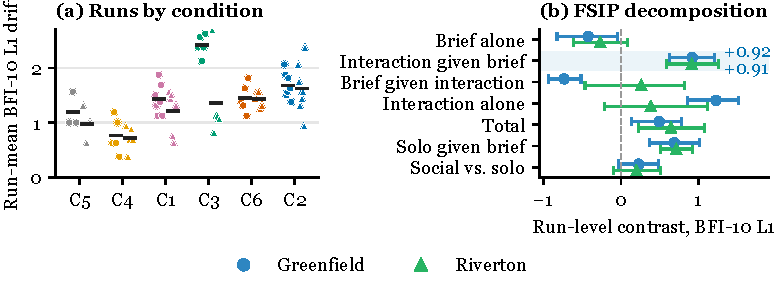
\includegraphics[width=\textwidth]{figures/fig4_primary.pdf}
\caption{Run-level drift (a) and FSIP decomposition (b). $C_2$ exceeds $C_4$ in both scenarios.}\label{fig:primary}
\end{figure}

\textbf{Finding 1: the pure-interaction contrast clears all three gates in both scenarios.} As Table~\ref{tab:decomp} shows, controlled clones with the same private-brief assignment but no interaction differ from clones with the same assignment and 30 rounds of interaction by $\bar{\Delta}{=}{+}0.917$ (Greenfield) and ${+}0.912$ (Riverton) BFI-10 L1 units, with exact run-level $p{=}0.0008$ and $0.0039$ and $g{\approx}1.0$ on both. Because BFI-10 L1 sums five factor-level absolute shifts, this corresponds to about 0.18 Likert points per factor. All eight Greenfield $C_2$ run means exceed the largest $C_4$ mean, and in Riverton seven exceed it and one ties it (Figure~\ref{fig:primary}a). The headline result does not depend on the thinner $C_5$ baseline. The two scenarios are topically disjoint (a community grant and a workforce transition). The BFI-10 items~\citep{Rammstedt2007_BFI10,PsychoBench} are unrelated to either scenario, and the magnitude is near-identical across them. This is the cross-task, cross-scenario stability signature that would be hard to obtain from any mechanism reducible to surface opinion change on the discussed topic.

\textbf{Finding 2: brief alone does not explain the drift.} A brief, a noisy no-interaction baseline, or a probe artifact could in principle produce the BFI-10 shift without interaction. Figure~\ref{fig:primary}b rules out the brief. The brief-alone contrast $(C_4){-}(C_5)$ is small and negative on Greenfield ($\bar{\Delta}{=}{-}0.43$) and trends negative on Riverton without significance. In contrast, $(C_2){-}(C_4)$ stands roughly $1.2{-}1.3$ BFI L1 units above the brief-alone row. Interaction without any brief asymmetry is also sufficient on at least one scenario, since $(C_3){-}(C_5)$ is significantly positive on Greenfield and trends positive on Riverton. Among the five FSIP contrasts, only $(C_2){-}(C_4)$ is positive, large, and significant in both scenarios.

The BFI-10 result remains a response-profile drift on a human-derived inventory, not evidence of human-like personality change. Still, three observations make trivial accounts too small. First, the headline contrast holds asymmetric briefs fixed. Second, the no-SRM ablation (RQ2) keeps the drift positive without the typed SRM extractor. Third, the same interaction protocol produces structured Decision and Prediction effects (RQ3--RQ5), which is not what one would expect from random sampling drift alone.

\subsection{RQ2: Does the Shift Survive Memory, Temperature, and Partner Changes?}\label{sec:exp-srm}

\begin{figure}[t]
\begin{minipage}[c]{0.56\textwidth}
\centering\footnotesize
\setlength{\tabcolsep}{2.4pt}
\captionof{table}{Setting ablations. Every contrast stays positive (raw $\bar\Delta$, exact $p$).}\label{tab:settings}
\begin{tabular}{llrrrr}
\toprule
& & \multicolumn{2}{c}{Greenfield} & \multicolumn{2}{c}{Riverton} \\
\cmidrule(lr){3-4}\cmidrule(lr){5-6}
Setting & Contrast & $\bar\Delta$ & $p$ & $\bar\Delta$ & $p$ \\
\midrule
\tableinput{tables/t2_settings.tex}
\bottomrule
\end{tabular}
\end{minipage}\hfill
\begin{minipage}[c]{0.41\textwidth}
\centering
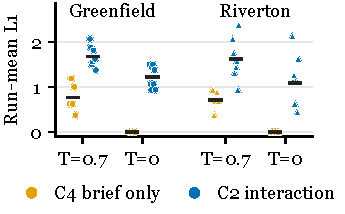
\includegraphics[width=\linewidth]{figures/fig5_t0.pdf}
\captionof{figure}{$C_2$ stays above $C_4$ at BFI $T{=}0.7$ and $T{=}0$.}\label{fig:t0}
\end{minipage}
\end{figure}

\textbf{Finding 3: the shift survives deterministic re-probing.} We re-probed every frozen primary $C_2$ and $C_4$ state at BFI temperature zero, without generating new interaction trajectories. The raw contrast remains $+1.227$ on Greenfield and $+1.094$ on Riverton (Table~\ref{tab:settings}), with all 8/8 $C_2$ run means positive in both scenarios (Figure~\ref{fig:t0}). At $T{=}0$, $C_4$ produces the same pre/post score under its identical prompt, giving a deterministic zero, so raw differences are the informative scale. The same leading signed factors keep 8/8 directional agreement: Greenfield extraversion $+0.344$ and neuroticism $+0.398$, Riverton agreeableness $-0.227$ and openness $-0.312$.

\textbf{Finding 4: the drift does not need the SRM extractor.} A faulty memory module could inject structure that later surfaces on response-profile probes, so we re-run $C_2$ and $C_5$ with SRM extraction disabled and verbatim conversation excerpts retained in the same memory interface (3 vs.\ 3 replicas per scenario). The no-SRM effect remains positive in both scenarios ($+1.708$ and $+0.958$). Both exact two-sided tests give $p{=}0.10$, the minimum attainable with 3 vs.\ 3 runs, so we present this ablation as exploratory evidence. Relative to the SRM-on production estimate for $(C_2){-}(C_5)$, disabling SRM enlarges the BFI effect from $g{=}{+}0.56$ to $g{=}{+}2.02$ on Greenfield and from $g{=}{+}0.62$ to $g{=}{+}0.94$ on Riverton. This pattern is consistent with typed memory acting as a stabilizing anchor rather than as the source of the signal. Because the check has 3 replicas per condition and no $C_4$, the stabilizing role remains open for a larger run-level study.

\textbf{Finding 5: solo generation bounds the mechanism.} As Table~\ref{tab:settings} and Figure~\ref{fig:primary}a show, $C_6$ mean drift is 1.450 on Greenfield and 1.425 on Riverton, between $C_4$ (0.762, 0.713) and $C_2$ (1.680, 1.625). The same $C_2{>}C_6{>}C_4$ ordering appears in both scenarios. Extended generation and history move $C_6$ above $C_4$ ($+0.688$, $p{=}0.0159$, and $+0.713$, $p{=}0.0079$). $C_2$ remains highest in both scenarios ($C_2{-}C_6{=}{+}0.230$ and ${+}0.200$, $p{=}0.143$ and $0.392$), leaving room for the additional contribution of reciprocal interaction. $C_6$ bounds this mechanism, while $(C_2){-}(C_4)$ remains the total interaction-given-brief contrast. Over the 30 rounds, belief-probe wording converges within groups in $C_2$ and $C_3$ but stays flat in $C_6$ and $C_1$ (Appendix~\ref{app:timecourse}).

\subsection{RQ3--RQ5: Does the SCT Route Hold from Decision to Transfer?}\label{sec:exp-decision}\label{sec:exp-prediction}

\begin{figure}[t]
\centering
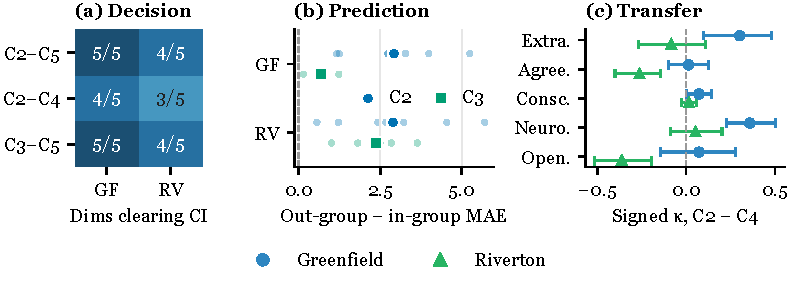
\includegraphics[width=\textwidth]{figures/fig6_route.pdf}
\caption{SCT route: clones diverge (a), predict exposed peers better (b), and transfer coherently (c).}\label{fig:route}
\end{figure}

\textbf{Finding 6 (RQ3): clones separate on the discussed task.} As Figure~\ref{fig:route}a shows, the $(C_2){-}(C_5)$ allocation contrast clears all five dimensions on Greenfield ($\bar g{=}{+}1.61$) and four of five on Riverton ($\bar g{=}{+}1.19$). The pure-interaction $(C_2){-}(C_4)$ row clears 4 of 5 dimensions on Greenfield and 3 of 5 on Riverton. This supports the SCT-Decision step. The agents first separate on the allocation problem, and the later off-topic probe is not an isolated psychometric blip.

\textbf{Finding 7 (RQ4): agents show an exposed-peer predictive advantage.} Each $C_2$ agent contributes one in-group MAE and one out-group MAE post-interaction. A one-sided paired Wilcoxon rejects the null in both scenarios. Greenfield has in-group MAE $4.18$ vs.\ out-group $7.10$ ($\Delta{=}{+}2.92$, $p{=}1.8{\times}10^{-8}$, $n{=}64$), and Riverton has $3.25$ vs.\ $6.15$ ($\Delta{=}{+}2.89$, $p{=}6.3{\times}10^{-10}$). The same contrast on $C_3$ is positive but smaller, with $\Delta{=}{+}0.69$ ($p{=}0.049$) and $\Delta{=}{+}2.36$ ($p{=}4.6{\times}10^{-5}$), as Figure~\ref{fig:route}b shows. The in-group target is an exposed peer, while the out-group target is absent from the predictor's conversation context. We therefore read this as an exposed-peer predictive advantage, with matched information access as the next control. Prediction is supporting evidence, and the primary BFI result stands on its own interaction control.

\textbf{Finding 8 (RQ5): the profile moves in coherent directions.} For each factor, $\kappa_f$ (Eq.~\ref{eq:drift}) compares post-minus-pre movement in $C_2$ and $C_4$ after reverse coding. Greenfield has $\kappa{=}{+}0.302$ for extraversion and ${+}0.358$ for neuroticism, both with 8/8 directional agreement across replicas, and ${+}0.072$ for conscientiousness with 7/8. Riverton has ${-}0.263$ for agreeableness (8/8) and ${-}0.362$ for openness (7/8), as Figure~\ref{fig:route}c shows. Greenfield's aggregate L1 variance ratio $C_2/C_4$ is 0.47, so its clearest factors move consistently while dispersion falls. Riverton's ratio is 4.11, a larger contribution from dispersion alongside consistent agreeableness and openness movement. The profile directions are therefore coherent and scenario-specific.

\subsection{RQ6: Does the Direction Hold Across Models, and What Does It Imply?}\label{sec:exp-cross}

\begin{figure}[t]
\centering
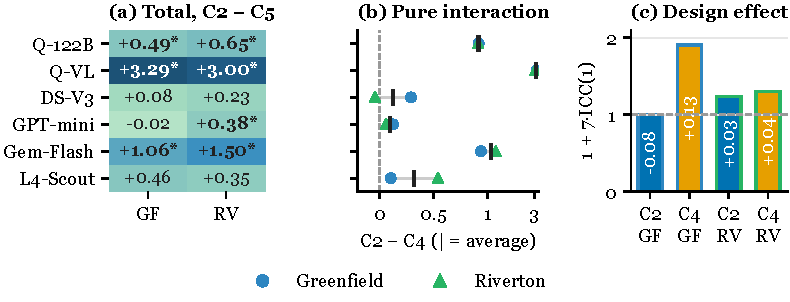
\includegraphics[width=\textwidth]{figures/fig7_breadth.pdf}
\caption{Cross-model breadth (a, b) and replicate dependence (c). All five $(C_2){-}(C_4)$ averages are positive.}\label{fig:breadth}
\end{figure}

\textbf{Finding 9: directional breadth is positive but uneven.} As Figure~\ref{fig:breadth}a shows, three of the five non-primary variants reach significance on $(C_2){-}(C_5)$ in at least one scenario. Qwen3-VL-32B and Gemini-2.5-Flash reach significance in both scenarios, and GPT-4.1-mini reaches significance on Riverton. DeepSeek-V3 and Llama-4-Scout do not reach significance. Under a no-effect null, ten scenario-by-variant cells tested at $\alpha{=}0.05$ would yield 0.5 positive cells in expectation. We observe five positive cells and no significant reversal. The smaller within-family Qwen3-VL-32B variant produces the largest raw drift ($\bar{\Delta}{\approx}3.0{-}3.3$), but its standardized $g$ is inflated by an unstable pooled SD on its own $C_5$ (Appendix~\ref{app:cross}).

\textbf{Finding 10: the pure-interaction contrast is positive for every variant on average.} We completed matched $(C_2){-}(C_4)$ runs for all five variants, three runs per condition and scenario (Figure~\ref{fig:breadth}b). All 5/5 model-level scenario averages are positive (one-sided exact sign test $p{=}0.031$). The panel includes DeepSeek-V3's near-zero, slightly reversed Riverton cell. A 3 vs.\ 3 two-sided exact permutation test has 20 possible allocations, so its minimum attainable $p$ is 0.10. The panel therefore provides directional breadth across the five tested controlled-clone configurations.

\textbf{Finding 11: uncertainty belongs at the simulation level.} OASIS-style populations are used to estimate group polarization and herd-effect trajectories, including normal-theory intervals over posts and comments within one simulated interaction process~\citep{OASIS}. Agents and posts that share an evolving history also share dependence. In our data, estimated agent-level ICC(1) ranges from $-0.079$ to $0.129$ across the four primary cells, and treating 8 agents as independent would overstate effective sample size by design factors up to 1.91 (Figure~\ref{fig:breadth}c). The practical correction is to keep the point estimate, recompute uncertainty at the independent simulation level, and check it against a no-interaction condition.

\subsection{RQ7: Does Transfer Extend Beyond BFI-10 in Riverton?}\label{sec:exp-scenario}\label{sec:exp-case}

\begin{table}[t]
\centering\footnotesize
\setlength{\tabcolsep}{3pt}
\caption{Gate status (A) and the Riverton route (B). BFI-10 is SCT-positive in both scenarios.}\label{tab:gates}\label{tab:riverton-case}
\begin{tabular}{l cc cc}
\toprule
\multicolumn{5}{l}{\textbf{(A) Gate status}, $\bar\Delta$ ($g$) with 95\% CI or Welch $p$} \\
& \multicolumn{2}{c}{Greenfield} & \multicolumn{2}{c}{Riverton} \\
\cmidrule(lr){2-3}\cmidrule(lr){4-5}
\tableinput{tables/t3_gates.tex}
\bottomrule
\end{tabular}

\vspace{4pt}
\begin{tabular}{P{0.13\textwidth}P{0.44\textwidth}P{0.38\textwidth}}
\toprule
\multicolumn{3}{l}{\textbf{(B) Riverton case study along the SCT route}} \\
Route step & Observed pattern & Interpretation \\
\midrule
Decision & $(C_2){-}(C_5)$ clears 4 of 5 allocation dimensions, $\bar g{=}{+}1.19$ & Interacting clones separate on the discussed budget task \\
Prediction & in-group MAE $3.25$ vs.\ out-group $6.15$, $\Delta{=}{+}2.89$, $p{=}6.3{\times}10^{-10}$ & Exposed-peer predictive advantage \\
Primary transfer & BFI-10 $(C_2){-}(C_4)$ gives $\bar{\Delta}{=}{+}0.91$, $g{=}{+}0.96$ & Off-topic response-profile drift survives the matched-brief control \\
Secondary transfer & conformity $g{=}{-}0.62$, consistency $g{=}{+}1.74$ on $(C_2){-}(C_4)$ & The strongest scenario also changes social-pressure and consistency probes \\
\bottomrule
\end{tabular}
\end{table}

\textbf{Finding 12: in Riverton, transfer extends beyond BFI-10.} The scenario asks an AI Transition Committee to allocate a \$5M budget across Automation, Workforce Training, Employee Support, Innovation Lab, and Data Infrastructure. Brief A emphasizes efficiency and technology infrastructure. Brief B emphasizes workforce readiness and employee support. Table~\ref{tab:gates}B shows how the same run family moves from topic-level divergence to peer modeling and then to off-topic transfer. Riverton is a boundary case, not a claim about all domains. Conformity is SCT-positive on Riverton but null on Greenfield ($g{=}{-}0.05$, $p{=}0.81$). Consistency on the same contrast is significantly positive on Riverton but null on Greenfield ($g{=}{+}0.01$). On Greenfield, the consistency lift on $(C_2){-}(C_5)$ is driven by the brief component $(C_4){-}(C_5)$ rather than by interaction. A reasonable account is that Riverton's workplace transition framing creates stronger group identification than Greenfield's community-grant framing, so effects that depend on in-group identification emerge more clearly. Wording consistency also concerns the allocation topic itself, so it cannot by itself establish off-topic transfer. We report the asymmetry rather than averaging it away.
